\section{Resultados} 
\label{posing:result}
%%%%%%%%%%%%%%%%%%%%%%%%%%%%%%%%%%%%%%%%%%%%%%%%%%%%%%%%%
\todo{No me gustan los apartados. Separa entre rendimiento y calidad}

\todo{pasiva}
En esta sección se procede a mostrar como el algoritmo propuesto es usado para transformar distintos modelos virtuales de la posición de reposo que presentan, hasta la posición deseada. Dentro de estos modelos se incluyen modelos comerciales, otros procedentes de imágenes de pacientes reales o ejemplos diseñados para probar el sistema como se puede ver a continuación:\todo{qué se puede ver a continuación?}
\begin{itemize}
    \item \emph{ZygoteBody}$^{TM}$ Masculino
    \item \emph{ZygoteBody}$^{TM}$ Femenino
    \item \emph{Anatomium} Masculino
    \item \emph{Segmented Inner Organs}\cite{VoxelMan}
    \item Datos de pacientes reales
    \item Modelo de barra con cuatro huesos
\end{itemize}

\todo{lo dejo aquí. Reescribe todo}
Estos modelos han sido utilizados para ilustrar los resultados de probar las diferentes técnicas de \emph{skinning} utilizadas en esta tesis. 

\begin{figure*}[h]%[b]%[b!ht]
  \centering
  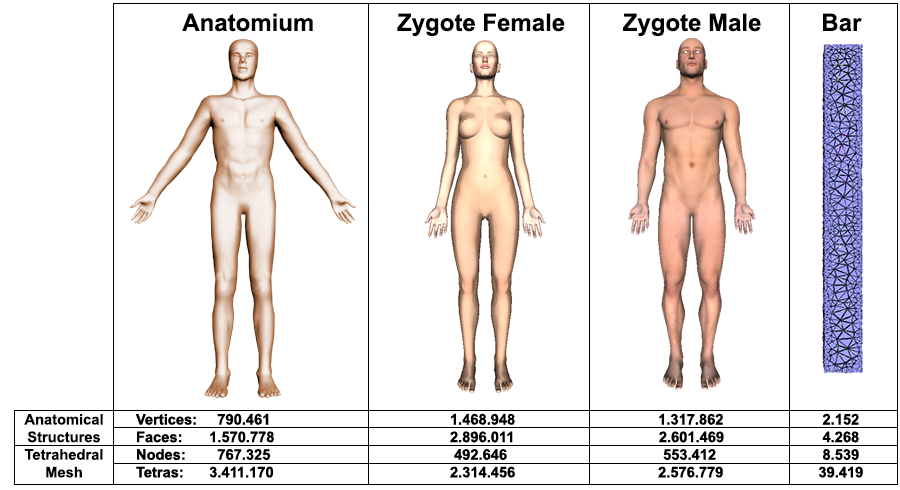
\includegraphics[width=0.90\textwidth]{IMG/models}
    \caption{Tamaño de los modelos usados en los test}
    \label{fig:models}
\end{figure*}

La figura ~\ref{fig:models} resume el tamaño de los modelos que se utilizarán y las mallas volumétricas asociadas a esos modelos. Es necesario remarcar las dimensiones de los modelos anatómicos y las representaciones volumétricas en comparación con los tamaños habituales vistos en la sección de estado del arte (ver sección \ref{art:animation}). En ocasiones, estos modelos tienen una complejidad de un orden de magnitud superior a las mostradas en la bibliografía.

Con el objetivo de no necesitar un usuario con habilidades artísticas o conocimientos avanzados de anatomía, se han utilizado animaciones procedentes de la base de datos de \ac{MoCap} de la \emph{Carnegie Mellon University}~\cite{CMUMCD}.

El computador utilizado para realizar todos los test de la presente tesis se compone de un procesador \emph{Intel\textregistered i7-4820K @ 3.7GHz}, tarjeta gráfica \emph{GeForce GTX 770} y 16GB de memoria \acs{RAM}.


\subsection{Proceso previo}
Como se ha descrito en la sección anterior, el algoritmo propuesto delega una serie de tareas a un proceso previo. Este proceso es realizado una vez por modelo y de las pruebas realizadas nunca ha excedido más de siete minutos. 


Hay que destacar que los modelos con los que se ha trabajado no están exentos de problemas. Por una parte, en ambos modelos de \emph{ZygoteBody}$^{TM}$ presentan auto-colisiones y se puede encontrar multitud de colisiones entre distintos tejidos. Además, zonas como la axila resultan zonas conflictivas como se puede observar en la figura \ref{fig:zygoteproblems}. 

Por otra parte, muchos de los procedimientos médicos se realizan en áreas localizadas, por lo tanto, muchas de las imágenes médicas disponibles no representan completamente el modelo anatómico del paciente. El algoritmo propuesto es capaz de tratar con información incompleta como podemos observar en la figura \ref{fig:patient} donde se muestra un modelo construido a partir de imágenes médicas reales.

\begin{figure}[h]
   \centering
    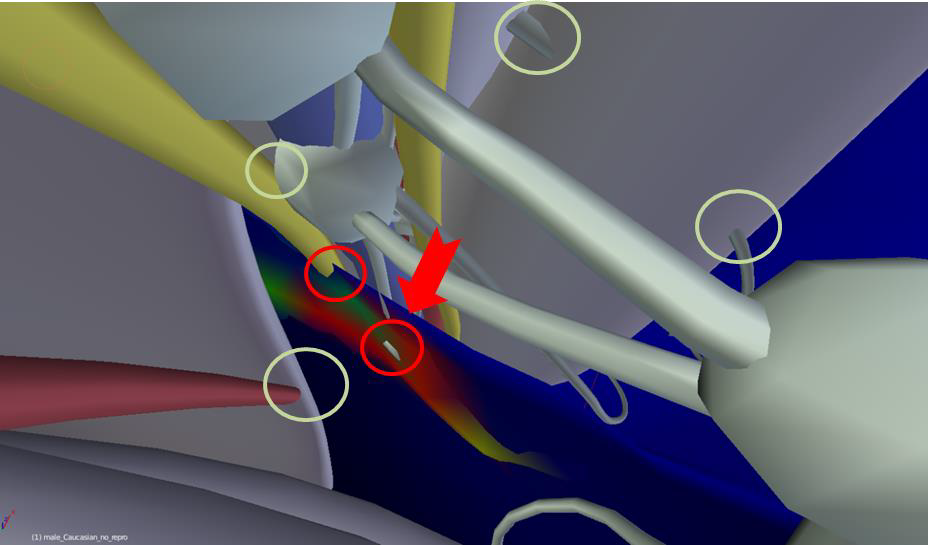
\includegraphics[width=0.5\textwidth]{IMG/zygoteproblems.png}
    \caption{Axila del modelo \emph{ZygoteBody}$^{TM}$ Masculino. Con círculos amarillos se observa colisiones entre diferentes tejidos. Los círculos rojos representan colisiones con el tejido de la piel  }
   \label{fig:zygoteproblems}
\end{figure}


%%%%%%%%%%%%%%%%%%%%%%%%%%%%%%%%%%%%%
\begin{figure}[h]
   \centering
    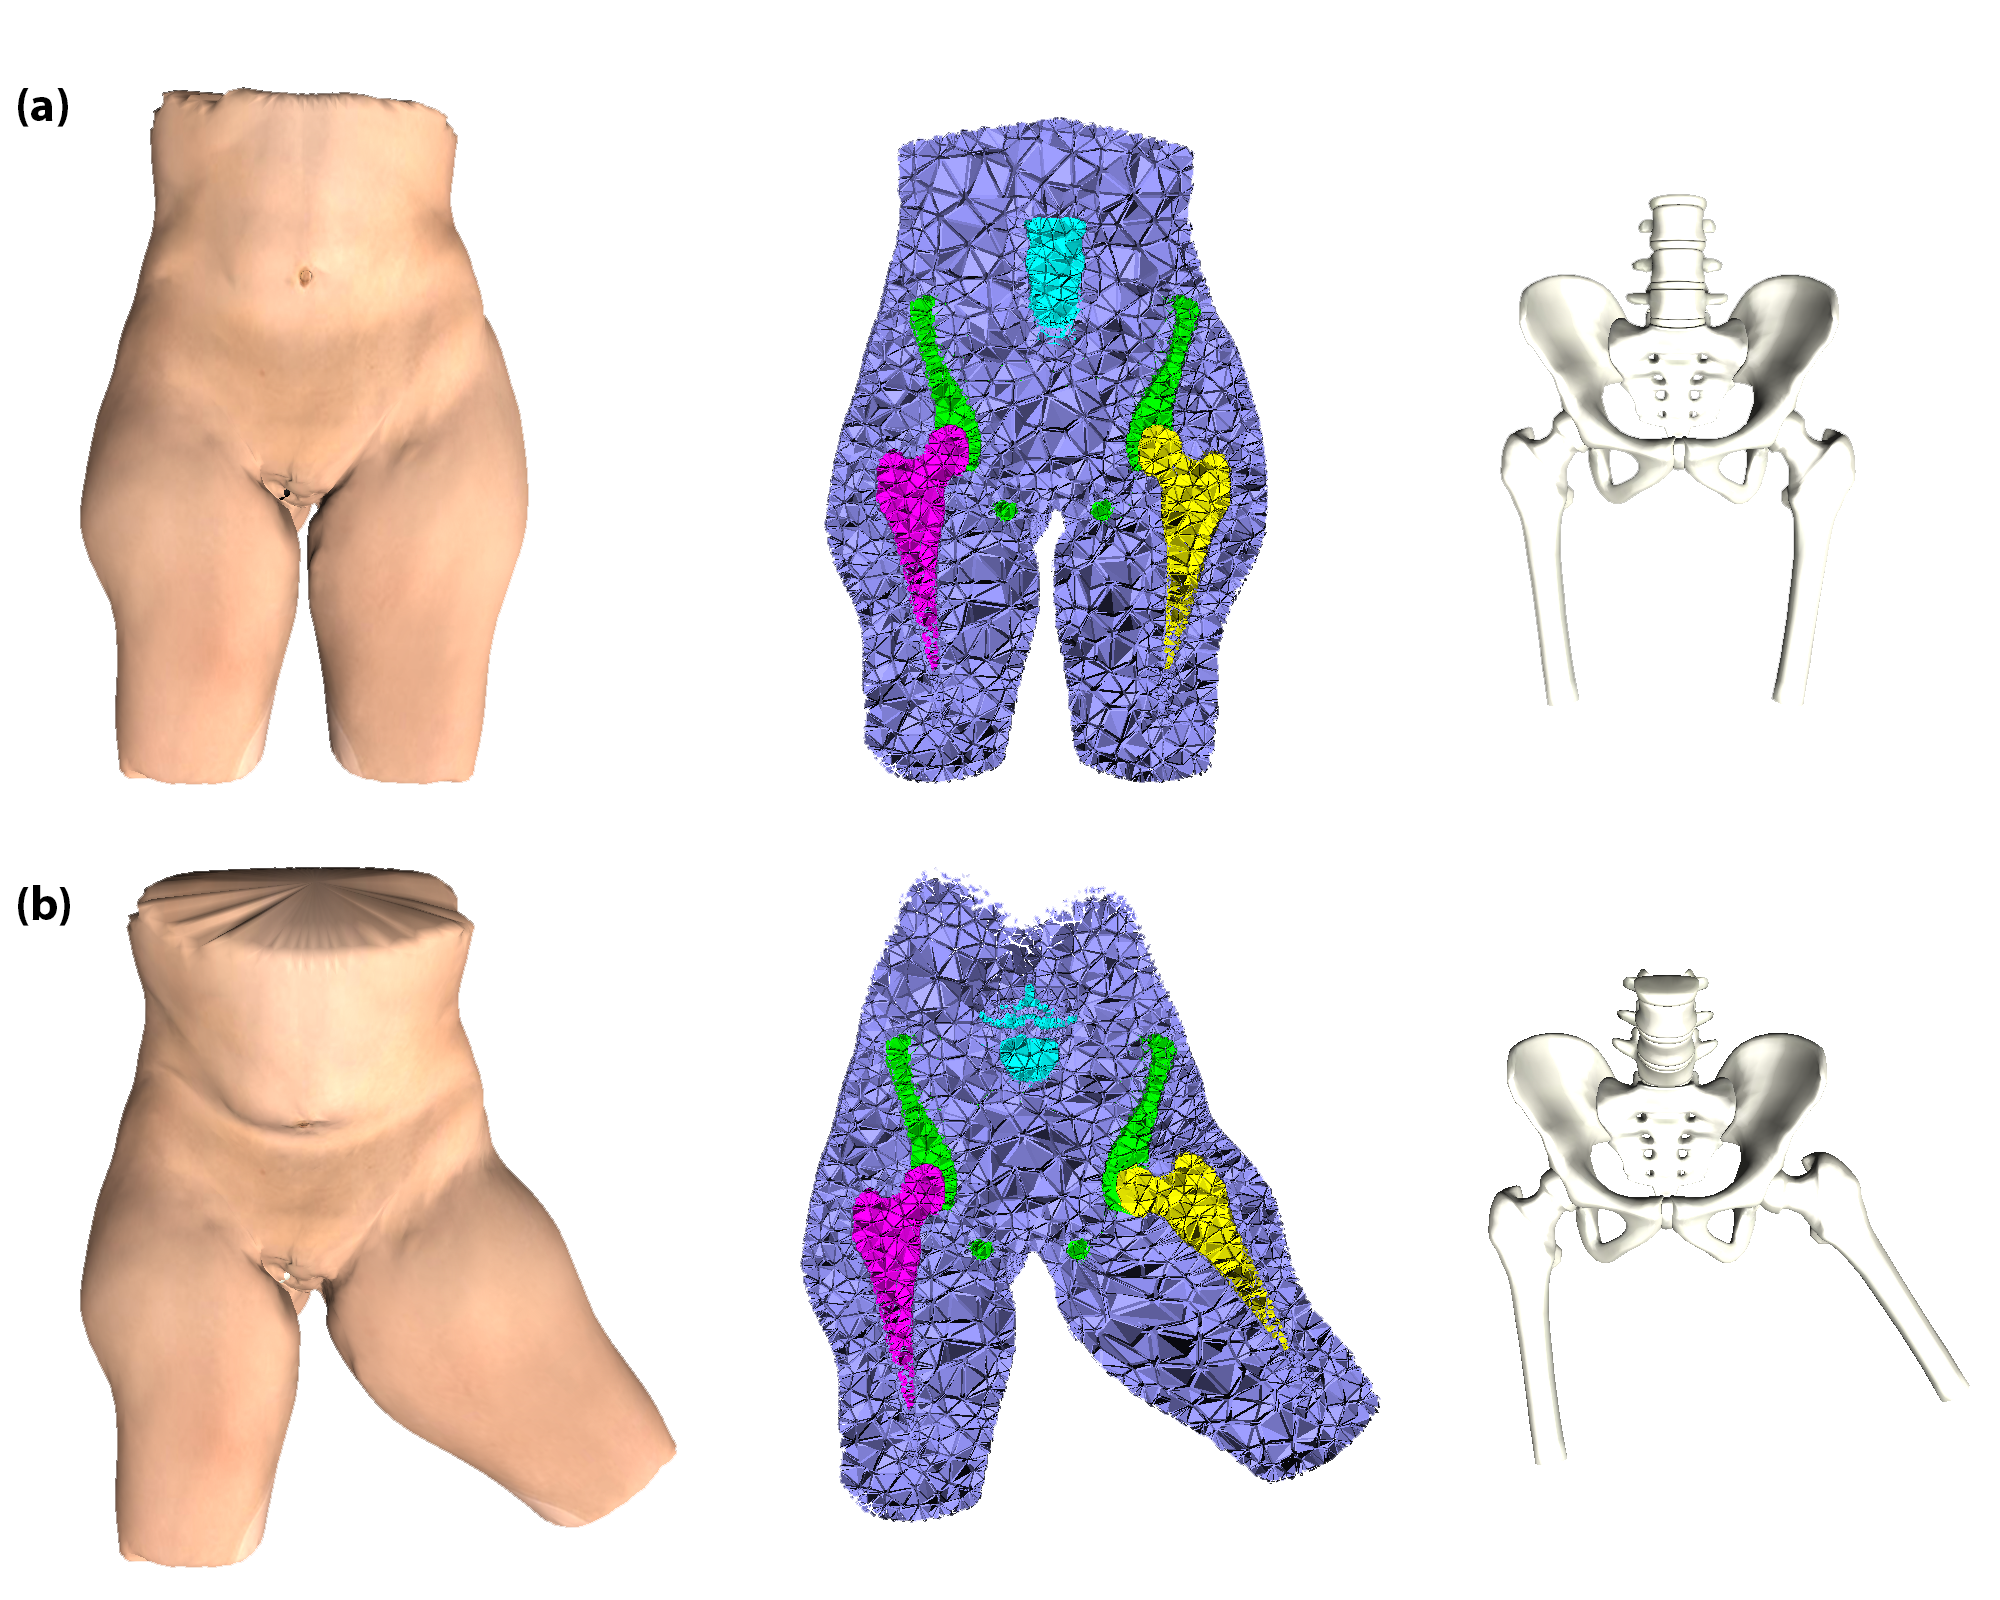
\includegraphics[width=0.5\textwidth]{IMG/patient.png}
    \caption{ La fila (a) muestra el paciente virtual construido a partir de datos de paciente real y se encuentran en posición de reposo. El algoritmo de posicionamiento permite modificar la pose de estos datos.
    }
   \label{fig:patient}
\end{figure}
%

Debido a la necesidad de que el algoritmo resulte robusto frente a los problemas comentados, se ha procedido a añadir diferentes ajustes en el algoritmo propuesto en varias de sus etapas.

En la etapa de \emph{volumetrización} (sec. \ref{posing:volumetrizacion}) se ha modificado la creación de la imagen volumétrica para borrar los \emph{vóxeles} etiquetados por el borde de la piel. Por tanto, en la figura \ref{fig:voxelizacion}.c se puede observar que los \emph{vóxeles} marcados como piel son desetiquetados con el objetivo de ser capaces de no crear tetraedros que conecten zonas del brazo y el pecho. En la figura \ref{fig:volsol} se puede observar la diferencia en la malla volumétrica. En la columna de la izquierda se muestra la \emph{voxelización} de la axila sin quitar los \emph{vóxeles} de la piel y en la columna de la derecha se puede observar que la zona de la axila esta correctamente.

\begin{figure}[h]
   \centering
    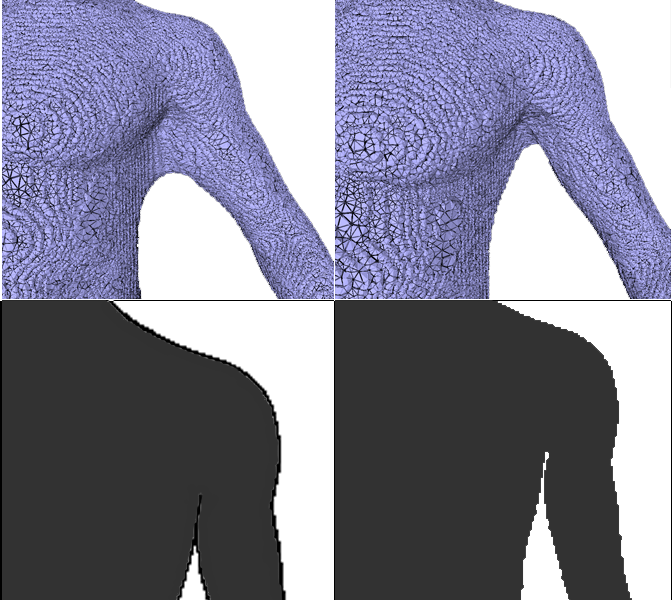
\includegraphics[width=0.45\textwidth]{IMG/volumetrizacion2.png}
    \caption{
    \emph{Volumetrización} de la zona de la axila. Columna izquierda muestra el problema de no eliminar los \emph{vóxeles} etiquetados como piel, en la columna de la derecha se resuelve el problema }
\label{fig:volsol}
\end{figure}


Con esta modificación se resuelve problemas de interconexión entre zonas no conectadas, aunque podría generar que se pueda encontrar tejidos que no están dentro de la malla volumétrica. Este problema sería adicional al que podría ocurrir donde el modelo que llega como entrada del \ac{TPTVPH} tuviera ciertos tejidos fuera de la piel. Debido a esto se ha propuesto una modificación de la etapa mapeado (ver sección \ref{posing:Mapeado}) para resolver este problema. Aprovechando la estructura espacial que proporciona la \ac{tabla hash}, aunque el vértice no esté dentro de ningún tetraedro, es fácil calcular el tetraedro más cercano para asociarle con él. Con esta modificación, en el caso concreto del modelo \emph{ZygoteBody}$^{TM}$ Masculino, alrededor de un 4.6\% de los vértices se encontrarían fuera de la malla volumétrica. 
Estos vértices no afectan de manera determinante en el proceso de mapeado. En este caso, el tiempo de mapeado es 36,35 segundos utilizando la \ac{tabla hash} como método de búsqueda. Este tiempo es muy pequeño si se compara con el tiempo que tardaría el proceso de mapear usando la técnica de fuerza bruta, que sería de 4 horas y 55 minutos para relacionar 1277325 de vértices a 2584115 de tetraedros en el caso del mismo ejemplo.  En la tabla \ref{tab:bruteforce} se muestra una comparación entre los tiempos empleados en mapear los distintos tejidos del \emph{ZygoteBody}$^{TM}$ Masculino con su malla volumétrica. Los modelos más complejos obtienen datos similares que se sitúan en torno a los cinco a siete minutos.


       
        
% \begin{landscape}
% \small
%  \centering % Center table
% \begin{center}
% \begin{tabular}{|c|c|c|c|c|c|  }
% \label{tab:forcebrute}

% \textbf{Modelo} & \textbf{Vértices} & \textbf{Vértices  huérfanos (\%)} & \textbf{Tetraedros (Elem./Vér.)} & \textbf{Spatial Hashing (ms)} & \textbf{Fuerza bruta (ms)} \\ 
% Skin                &32748      &89.81  &2,584,115 /555,702 &10678* &547967\\ 
% Muscles             &311600     &2.02   &2,584,115 /555,702 &12157* &4088365\\ 
% Nerves              &379008     &1.41   &2,584,115 /555,702 &12814* &5140770\\ 
% Connective Tissue   &168343     &0.68   &2,584,115 /555,702 &7881*  &2210942\\ 
% Lymphatic System    &5324       &5.66   &2,584,115 /555,702 &5456*  &702087\\ 
% Circulatory System  &380302     &4.29   &2,584,115 /555,702 &11541* &5008874\\ 
% TOTAL               &1277325    &4.6    &2,584,115 /555,702 &36.357103 &17.7*106 \\


% \end{tabular}.
% \caption{Brute force approach vs. spatial hashing approach.}
% \end{center}
% \normalsize
% \end{landscape} 




\todo{tabla enorme, como lo meto?}

Para finalizar de describir el proceso previo del algoritmo, a continuación se muestra la tabla \ref{tab:pre_pro} dónde se pueden consultar el tiempo empleado de cada etapa utilizando algunos de los modelos propuestos. 

\todo{meter todos los valores significativos de configuración}

Los valores de configuración para las distintas etapas son las siguientes:
La volumetrización no se hará en una caja contenedora más grande de tamaño 250x700x120. En cuanto a la función de similaridad empleada en la técnica de \emph{skinning} \ac{COR}, el valor de $\sigma$ que se utiliza es $0.1$.



\begin{table*}[!h]
\centering
\caption{Tiempo en milisegundos utilizado por cada etapa. ZM es Zygote Masculino, ZF es Zygote Femenino, A es Anatomium y CoR es la etapa de calcular los centros de rotación (sec. \ref{posing:Poses}).}
\begin{tabular}{cccccc}
\hline
\textbf{Modelo} & \textbf{Rigging} & \textbf{Volumetrización} & \textbf{Pesado} & \textbf{Mapeado} & \textbf{CoR }  \\ 
\hline
ZM  & 32698 & 69044 & 11762  & 51160   & 138005 \\ 
\hline
ZF  & 33251 & 63401 & 9171  & 71635   & 208886  \\ 
\hline
A   & 31891 & 120465 & 23318 & 44521  & 115214\\ 
\hline
\end{tabular}
\label{tab:pre_pro}
\end{table*}



\subsection{Selección de poses}

Con el objetivo que la selección de poses pueda ejecutarse en tiempo real, el proceso previo realiza las etapas más costosas computacionalmente que darán como resultado una serie de datos que serán usados por la herramienta al seleccionar el modelo virtual asociado. 

La etapa de selección de poses del algoritmo incluye la fase de \emph{skinning} para los vértices de los tetraedros y la consecuente deformación que es transferida a los tejidos del modelo virtual. Para mostrar de manera simple las diferencias visuales que se generan a través de las tres técnicas anteriormente citadas, se va a utilizar un modelo simple de un prisma rectangular con cuatro huesos virtuales en su interior. Este modelo por su simplicidad se utilizará para mostrar los resultados de rotaciones y giros para poder comparar entre técnicas utilizadas. En la figura \ref{fig:bar_bending} se pueden observar las diferencias visuales del método seleccionado (\ac{COR}) frente a los 2 métodos clásicos más conocidos en la literatura que son \ac{LBS} y \ac{DQS}. En cuanto a las rotaciones, se puede apreciar que en el caso de \ac{LBS} la articulación pierde volumen, sin embargo, en \ac{DQS} se puede observar un aumento de volumen. Respecto a los giros, es conocido que la técnica \ac{DQS} solventa el problema de \ac{LBS} donde la interpolación de los vértices se realiza de forma lineal produciendo el efecto \emph{candy-wrapper}. Así que, la técnica \ac{COR} es más robusta a cambios de volumen en rotaciones y además maneja adecuadamente los giros de las articulaciones. En esta figura se utilizan los tetraedros como referencia visual mostrando con los colores el pesado mostrado las diferentes influencias de los huesos virtuales. Se ha usado un código de colores, donde el color azul resultar ser los huesos impares que tienen influencia de 1 y el color rojo es donde los huesos pares tienen influencia de 1. Con este código de colores se puede observar las transiciones entre huesos.

\begin{figure*}[h]%[b]%[b!ht]
  \centering
  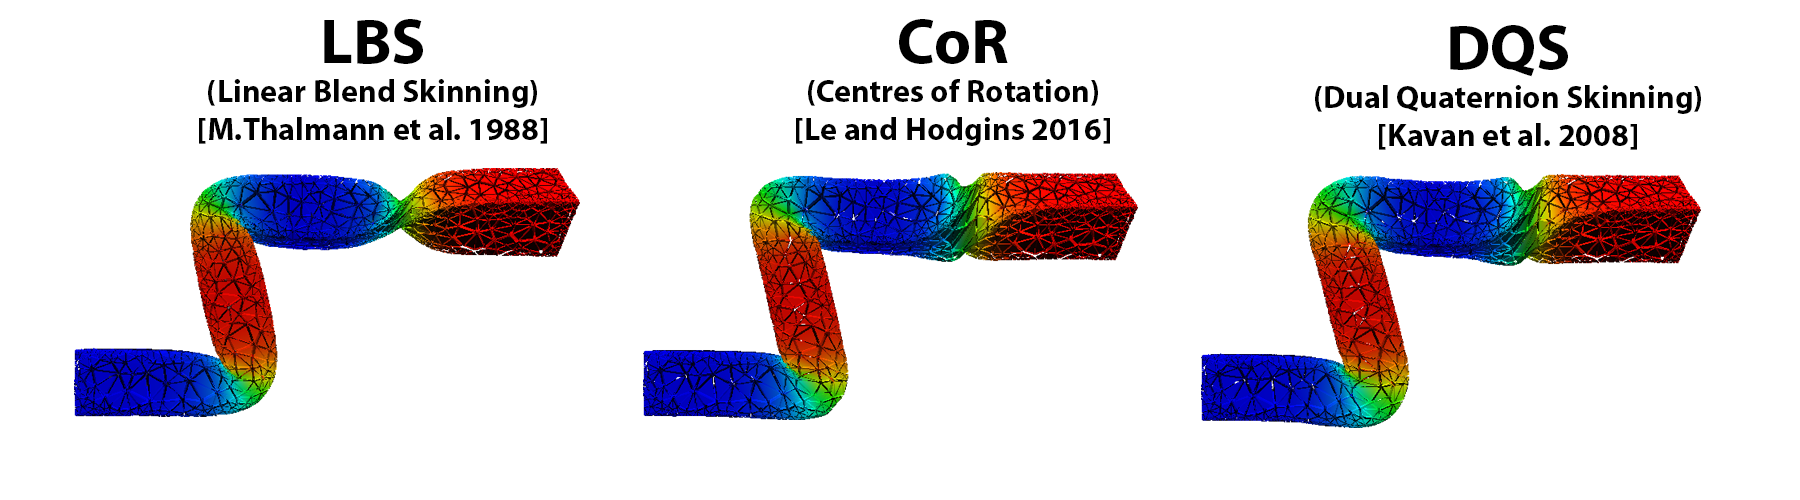
\includegraphics[width=0.90\textwidth]{IMG/BarraCoR}
    \caption{Deformación del prisma por las 3 técnicas. Primera rotación de 100º, segunda rotación de -100º y un giro de 135º.}
    \label{fig:bar_bending}
\end{figure*}
%%%%%%%%%%%%%%%%%%%%%%%%%%%%%%%%%%%%%

Una vez ilustradas las diferencias de manera teórica, a continuación se mostrarán las diferencias entre las distintas técnicas de \emph{skinning} utilizando los modelos anatómicos. En las siguientes figuras, se utilizará diferentes posturas de los modelos anatómicos para mostrar las diferencias en los resultados que producen cada uno de los métodos al deformar el paciente virtual.

En la figura \ref{fig:thigh_bending} se muestra una rotación de la articulación de la pierna. Las zonas perceptibles de producir artefactos son la zona superior del muslo en la zona inguinal y el glúteo. En esta imagen se puede observar que tanto la zona inguinal y el glúteo con la técnica \ac{LBS} produce una pérdida de volumen. En el caso de utilizar \ac{DQS} se aprecia el aumento de volumen predicho para esta técnica, sin embargo la técnica seleccionada \ac{COR} da como resultado un compromiso entre ambas técnicas. La imagen se acompaña con el tejido muscular en reposo como referencia y los tejidos circulatorio y nervioso de como el algoritmo propuesto es capaz de lidiar con toda aquella anatomía interna del modelo. En este ejemplo en concreto, las diferencias visuales entre técnicas de estos dos tejidos es mínimo al ser estructuras filiformes. 





% %%%%%%%%%%%%%%%%%%%%%%%%%%%%%%%%%%%%%
\begin{figure*}[h]%[b]%[b!ht]
  \centering
  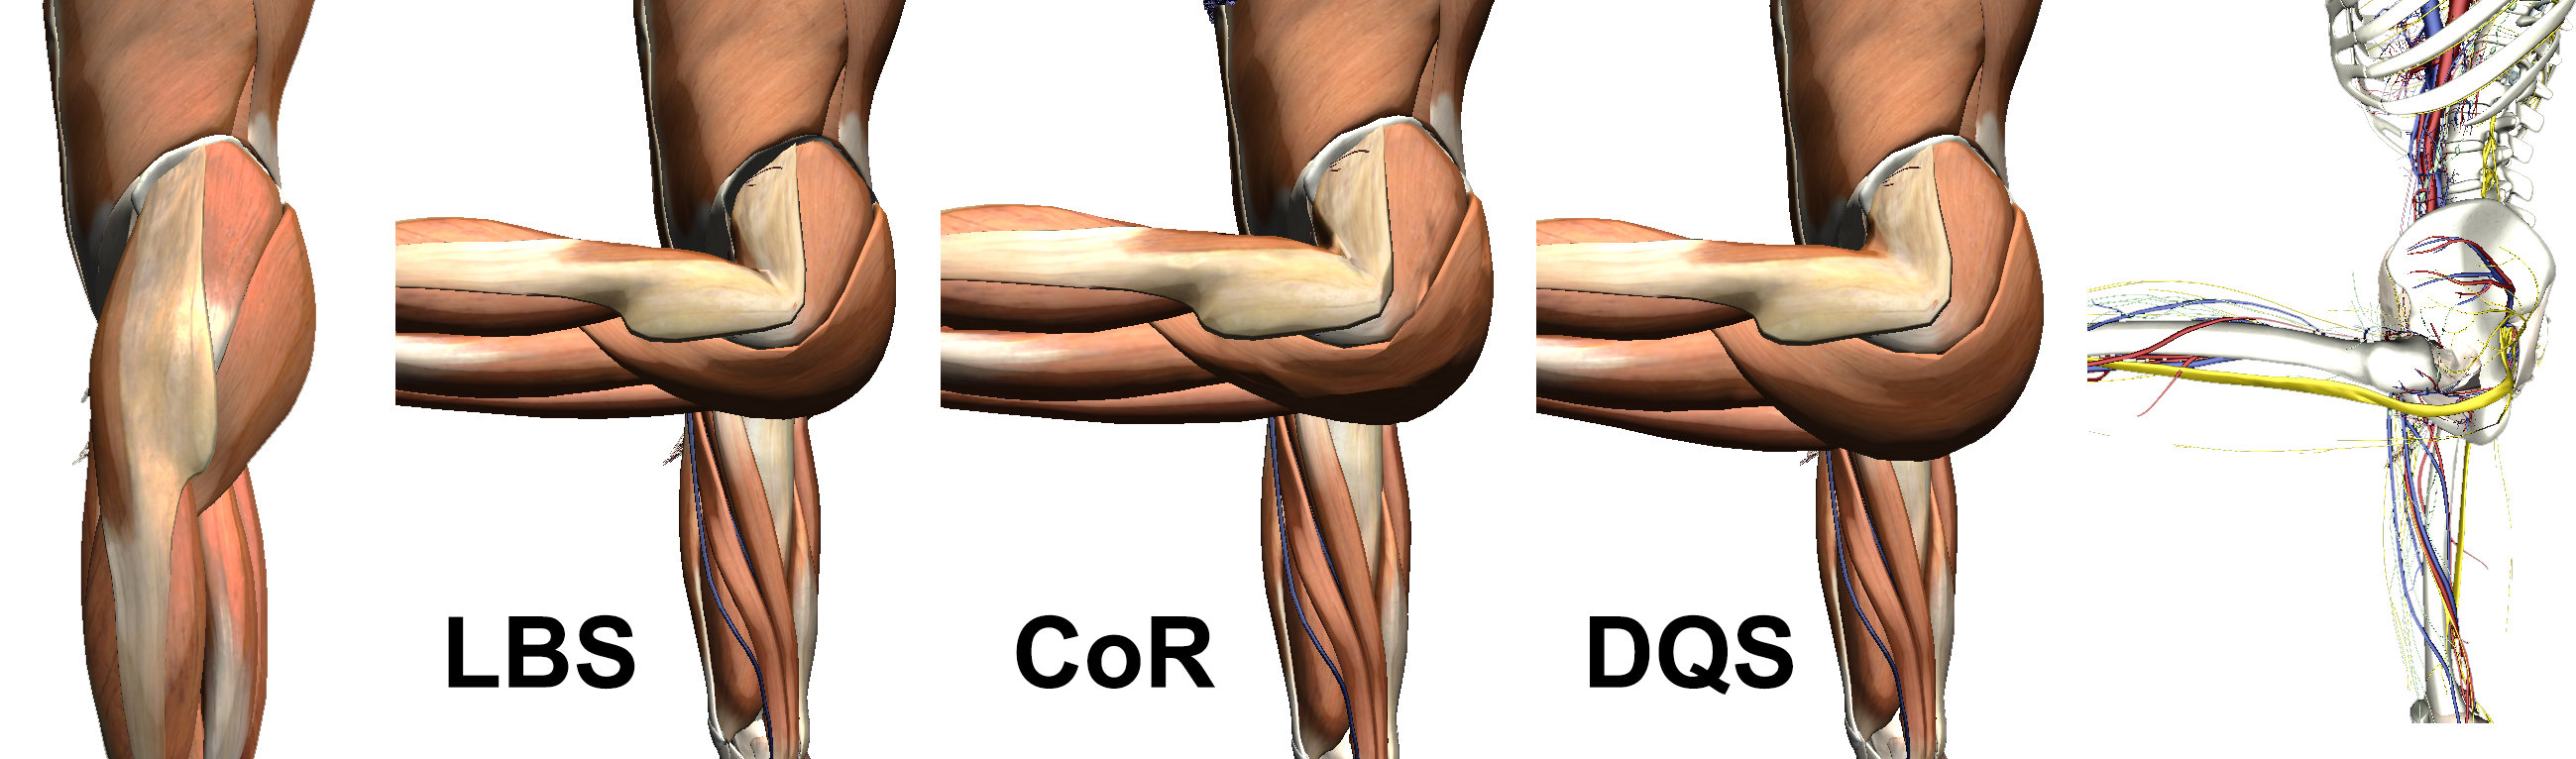
\includegraphics[width=0.90\textwidth]{IMG/compculo}
    \caption{ Deformación de una pierna. Izquierda: posiciones de los músculos en reposo; en el medio se muestran la pierna rotada usando las 3 técnicas de \emph{skinning} (\ac{LBS} pierde volumen tanto en el gluto como en la zona inguinal, \ac{DQS} añade volumen y \ac{COR} suaviza esos defectos; a la derecha podemos ver otros tejidos deformados.}
    \label{fig:thigh_bending}
\end{figure*}

\todo{más ejemplos aqui}
%%%%%%%%%%%%%%%%%%%%%%%%%%%%%%%%%%%%%

 Como se puede deducir de los requisitos descritos y la motivación de la presente tesis, se pretende que esta fase sea interactiva y el método debe ser capaz de manejar una gran cantidad de tetraedros (incluso con el gran tamaño de los ejemplos seleccionados). La tabla \ref{tab:inter} muestra el rendimiento  del método seleccionado (\ac{COR}) frente a los 2 métodos clásicos más conocidos en la literatura que son \ac{LBS} y \ac{DQS}. Como se puede observar, el rendimiento entre las diferentes técnicas son muy similares. La tabla muestra los valores máximos y mínimos de imágenes por segundo que es capaz de generar el algoritmo utilizando un ciclo de caminado para animar al modelo virtual.
%
\begin{table}[h]
\centering
\caption{Valores máximos y mínimos de imágenes por segundo durante el ciclo de caminado en la etapa de \emph{selección de poses} }
\begin{tabular}{cccc}
%\multirow{2}{*}{\textbf{Model}} & \multicolumn{2}{c}{\textbf{Interactive stage}} & \multirow{2}{*}{\textbf{Optimization}} \\
\textbf{Modelo}&\textbf{LBS} &\textbf{DQS} &\textbf{CoR} \\ 
\hline
ZM  & 111-90 & 100-90 & 100-76\\ 
\hline
ZF  & 76-60  & 66-52   & 60-50 \\ 
\hline
A   & 166-142 & 166-125 & 142-100\\ 
\hline
\end{tabular}
\label{tab:inter}
\end{table}


Con los resultados obtenidos, se puede afirmar que el algoritmo propuesto obtiene deformaciones visualmente realistas y es capaz de realizarlas en tiempo de ejecución delegando las etapas más pesadas a un proceso previo.

Finalmente, en la imagen \ref{fig:run1} se muestran resultados adicionales del uso del algoritmo con la técnica de \emph{skinning} \ac{COR} en los modelos \emph{ZygoteBody}$^{TM}$ Masculino y Femenino en diferentes situaciones.

%%%%%%%%%%%%%%%%%%%%%%%%%%%%%%%%%%%%%
\begin{figure*}%[h]%[b]%[b!ht]
   \centering
   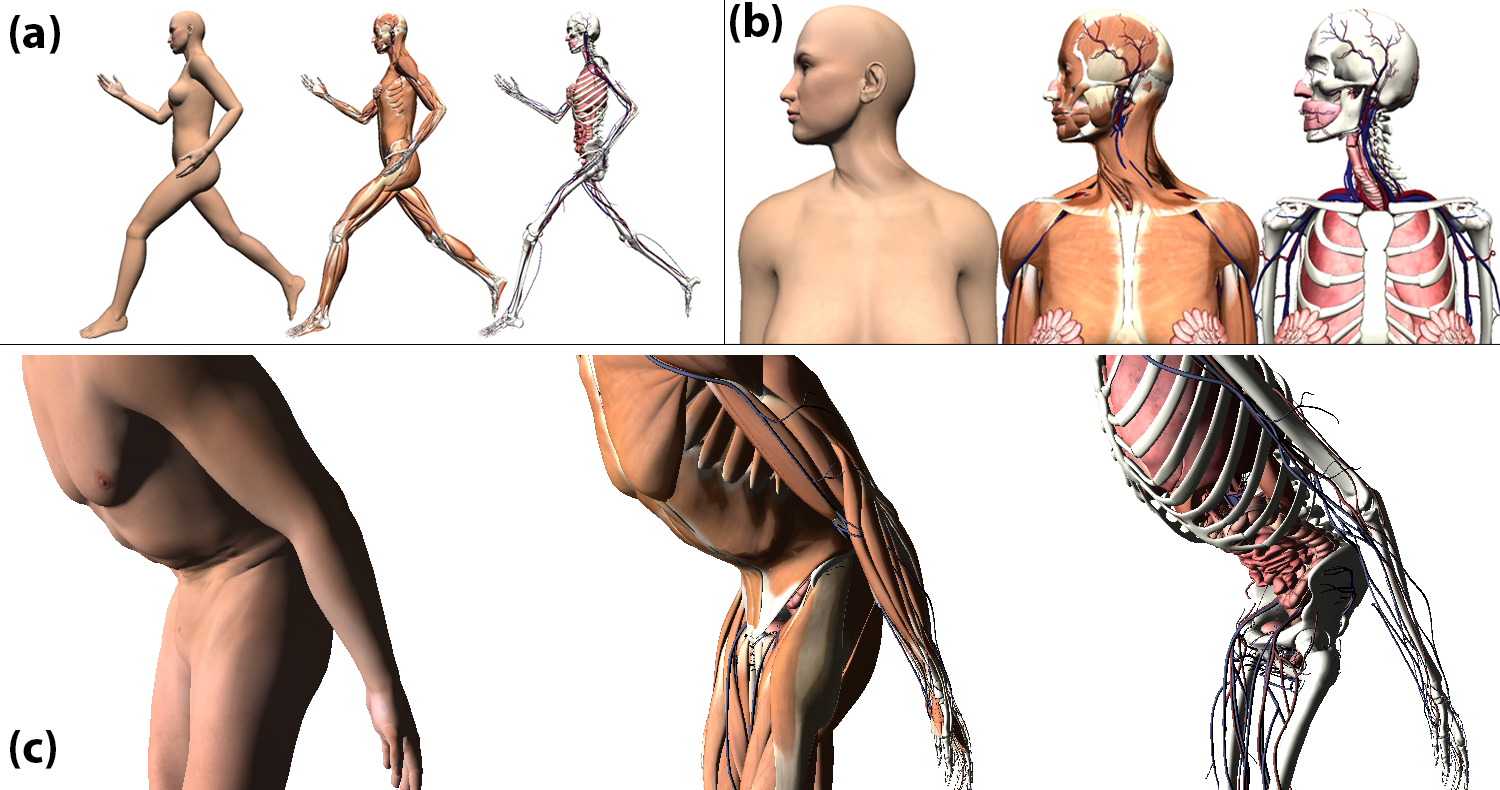
\includegraphics[width=0.90\textwidth]{IMG/examples}
    \caption{Resultados obtenidos utilizando \ac{COR}. (a): fotograma del ciclo de correr en el modelo ZF. (b): Cuello girado del modelo ZF. (c): Zona abdominal flexionada del modelo ZM.}
    \label{fig:run1}
\end{figure*}
%%%%%%%%%%%%%%%%%%%%%%%%%%%%%%%%%%%%%

\subsection{Optimización}

Las deformaciones resultantes de la etapa anterior dan como resultado poses visualmente realistas en la mayoría de los casos. La fase de \emph{skinning} basada en \ac{COR} solventa de forma efectiva los problemas típicos de las técnicas basadas en \ac{LBS} y de \ac{DQS}. Aún así, en algunas circunstancias se ha detectado un cambio no deseado de volumen. 
La técnica \ac{COR} no puede asegurar la conservación de volumen tal y como lo hacen las técnicas basadas en física. En esta sección, se va a comparar \ac{COR} con un modelo físico. Debido a que no se puede asegurar una apropiada descripción mecánica de los tejidos, el objetivo de esta optimización es garantizar la conservación del volumen.  Se ha propuesto utilizar la formulación \ac{FEM} co-rotacional para resolver el problema estático considerando un material lineal, isotrópico y homogéneo. En la mayor parte de los casos probados, con una iteración se obtenían resultados prácticamente indistinguibles de los resultados obtenidos con más iteraciones. 
 
%  Besides, the deformations are measured using the \emph{Cauchy} strain tensor. The boundary conditions, needed to solve the steady-state problem, are given by the positions of the vertices labelled as bones. The co-rotational formulation calculates the internal forces caused by the deformations in a non-rotated configuration. Then, the internal forces are rotated again into the final configuration \cite{Muller2004}. The algorithm needs to compute the element rotations in the final configuration. For this purpose, the solution is refined iteratively. The elastic used model can be tuned with two parameters: the \emph{Poisson ratio}  and the \emph {Young module}. The \emph{Poisson ratio} controls the volume conservation and it should take a value close to 0.5 (the real value has to be lower to ensure numeric stability). Since the material is homogenous, this value has no impact on the outcome. 
 Se ha escogido el módulo de \emph{Young}  intentado mejorar la estabilidad del sistema. Para ello, se han analizado distintas matrices de coeficientes del sistema, obtenidas a partir de distintos valores del módulo de \emph{Young}, quedándose con el valor que daba como resultado la matriz de coeficientes con menor número condicionante.
 
 La figura \ref{fig:anatomium} ilustra un ejemplo de cómo la técnica basada en la formulación \ac{FEM} soluciona alguna de los problemas de volumen que aparece con las otras técnicas. Sin embargo, debido a que la técnica \ac{COR} muestra buenos resultados se ha procedido a comprobar si esta optimización es elegida por los usuarios frente a la técnica geométrica.
 
 \begin{figure}[h]%[b]%[b!ht]
   \centering
   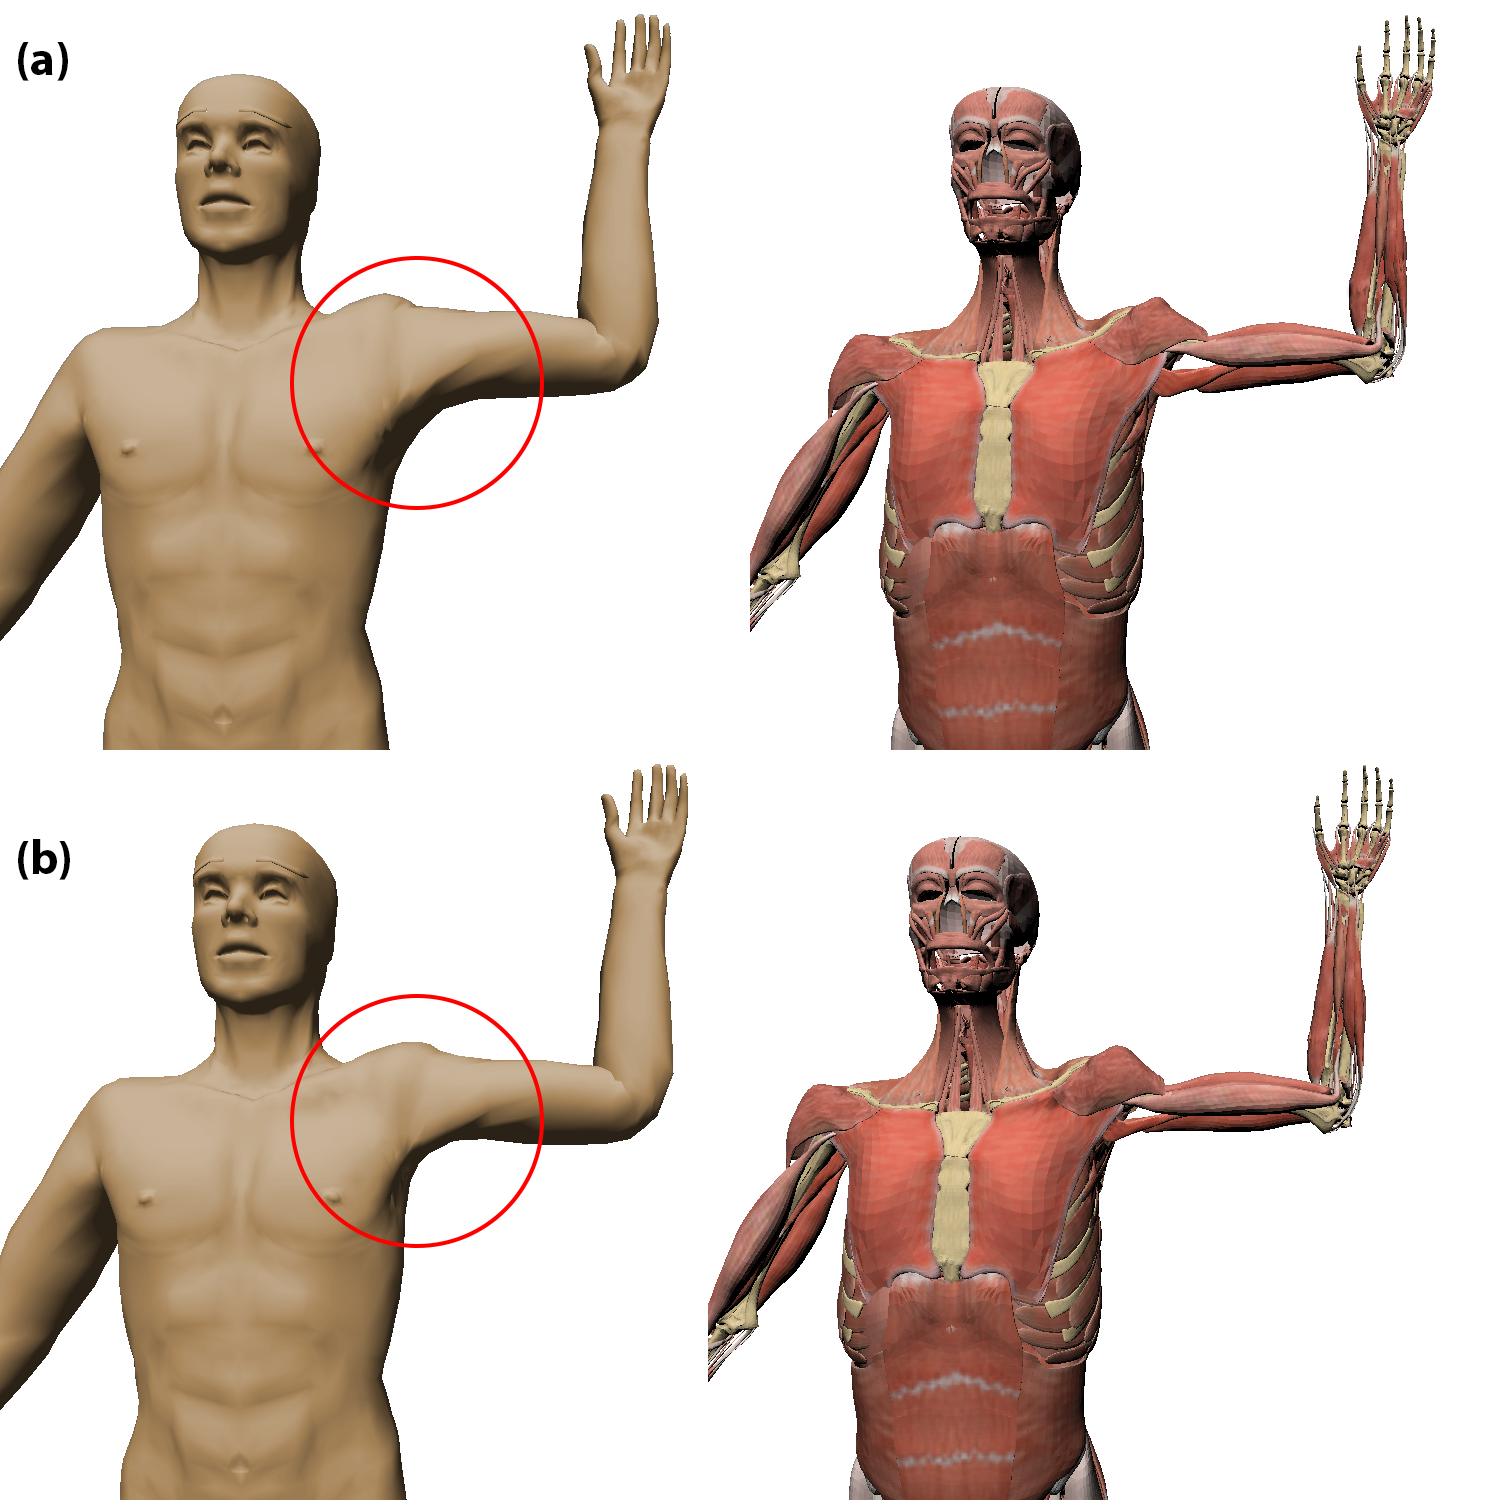
\includegraphics[width=0.45\textwidth]{IMG/AntCOR}
    \caption{ Comparación entre \ac{COR} (a) y el método \ac{FEM} (b)diseñado para conservar el volumen. \ac{COR} incrementa ligeramente el volumen en la zona de la axila.}
    \label{fig:anatomium}
\end{figure}
 
 Para probar esta hipótesis, se ha procedido a realizar una encuesta entre distintos usuarios. Un total de 16 sujetos han participado en la encuesta que se puede encontrar en los anexos \label{anexo:cuestionario1} y \label{anexo:cuestionario2}. 2 mujeres y 14 hombres, edad comprendida entre los 20 y los 52; 13 de ellos se han declarado profesionales de informática gráfica. En estas encuestas los participantes se les ha pedido que valoren el realismo presentado en unas imágenes estáticas. Estos sujetos debían contestar a una serie de preguntas, basándose en una escala de tipo  \emph{Likert} comprendida entre los valores 1 y 8. Las imágenes muestran seis posiciones diferentes y varios modelos y tejidos, donde la mitad de ellos han sido creados con la optimización \ac{FEM} y la otra mitad con la técnica \ac{COR}. Primero se ha mostrado la imagen de referencia para cada deformación y después se presenta de manera aleatoria las deformaciones con \ac{FEM} y \ac{COR}.

\todo{Marcos ayuda aquí} La asunción de homocedasticidad The assumption of homoscedasticity holds but normality does not.  Se han comparado los resultados obtenidos usando una prueba no paramétrica para muestras relacionadas. Los resultados de las muestras confirman que las diferencias entre ambos modelos no son significativas (\emph{p-value} $> 0.9$ intervalo de confianza).   A continuación, la figura \ref{fig:stat} muestra los resultados obtenidos. 
%

%
\todo{Metemos la gráfica de la otra encuesta?}
\begin{figure}[h]%[b]%[b!ht]
   \centering
   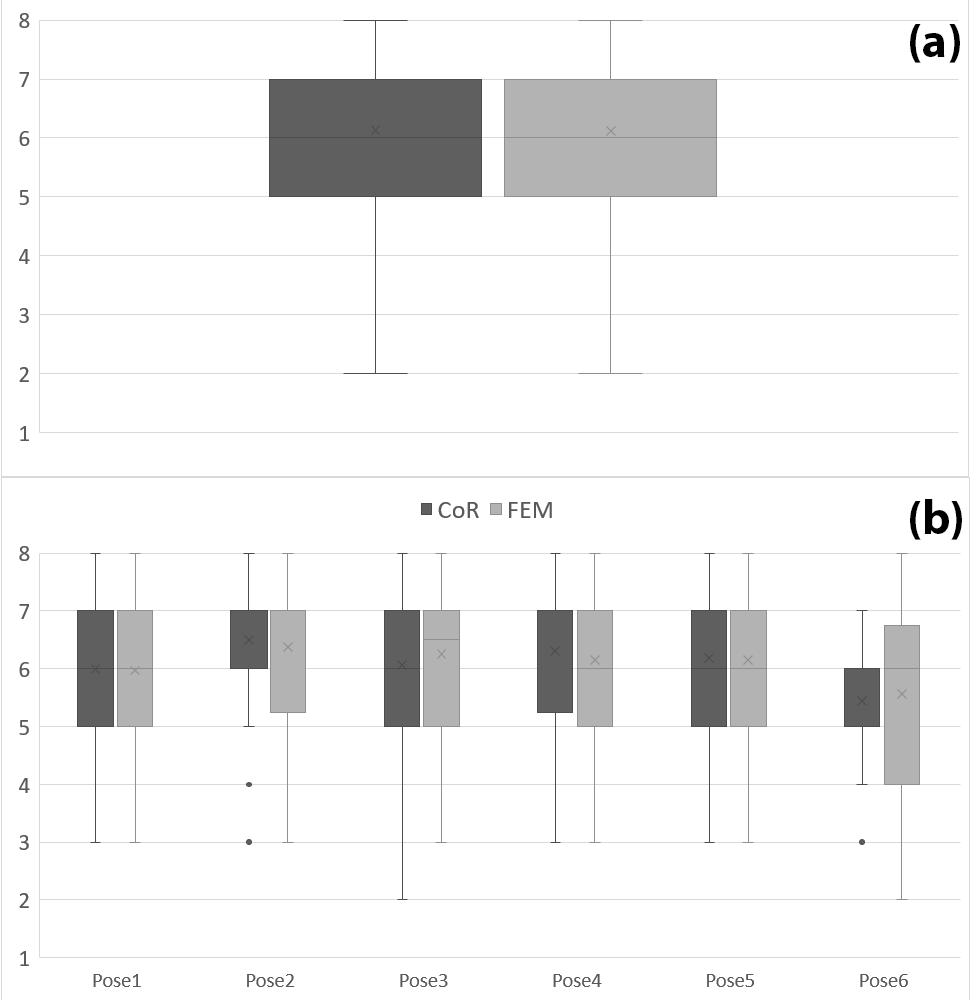
\includegraphics[width=0.45\textwidth]{IMG/boxplot}
    \caption{ Gráficas de cajas de bigotes comparando los resultados de la encuesta. Gráfica (a) muestra el resultado global, mientras la gráfica (b) compara el resultado obtenido por cada pose diferente.}
\label{fig:stat}
   \end{figure}

%%%%%%%%%%%%%%%%%%%%%%%%%%%%%%%%%%%%%

\subsection{ Animación de representaciones volumétricas}

\begin{figure*}[!ht]%[b]%[b!ht]
   \centering
   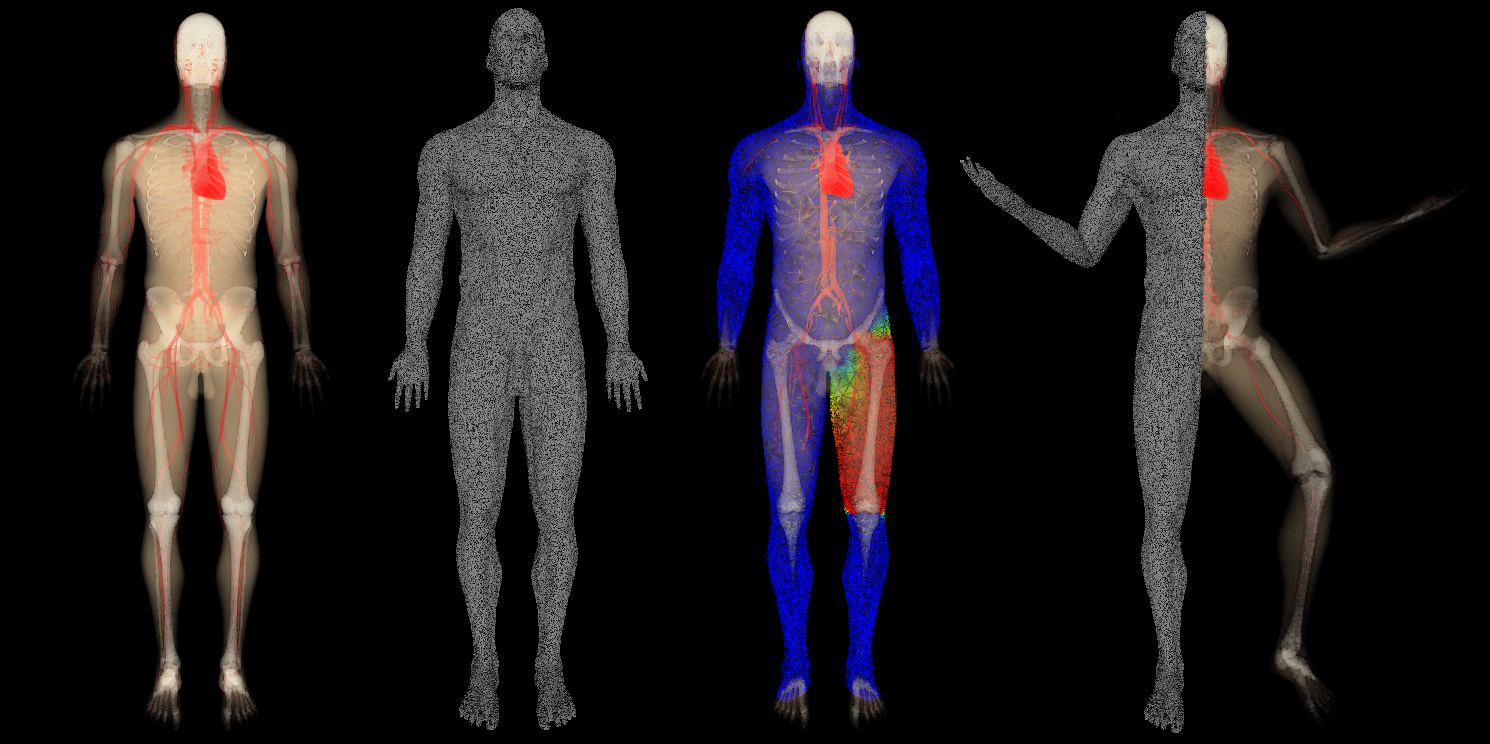
\includegraphics[width=0.90\textwidth]{IMG/Volumetric}
    \caption{Proceso de animación para modelo volumétrico. De izquierda a derecha: (1) modelo volumétrico en reposo, (2) malla de tetraedros generada, (3) malla de tetraedros representando el peso del fémur como ejemplo (rojo significa influencia cerca de 1, azul influencia 0) y (4) malla de tetraedros superpuesta al modelo volumétrico deformado. }
    \label{fig:volEx}
\end{figure*}
\todo{explica el por qué: el campo de desplazamientos}
La figura \ref{fig:volEx} muestra como puede ser utilizado el algoritmo propuesto a representaciones volumétricas de pacientes virtuales. En vez de transferir los pesos directamente de los tetraedros a los vértices interiores de los tejidos, se define un campo de desplazamientos que se puede usar para transformar tanto vértices de representaciones superficiales como para usarlo con \emph{vóxeles}. En este último caso, se definen una serie de \emph{píxeles} dentro de cada tetraedro en la posición deformada. Después son mapeados a la configuración de reposo utilizando la transformación inversa del campo de desplazamiento. Se itera sobre cada caja contenedora de la \ac{tabla hash} y se utilizan las coordenadas baricéntricas. Este proceso al ser fácilmente paralelizable en \ac{GPU} permite que se pueda \emph{renderizar} en tiempo real.
%


%%%%%%%%%%%%%%%%%%%%%%%%%%%%%%%%%%%%%
\begin{figure}[!ht]%[h]%[b]
   \centering
   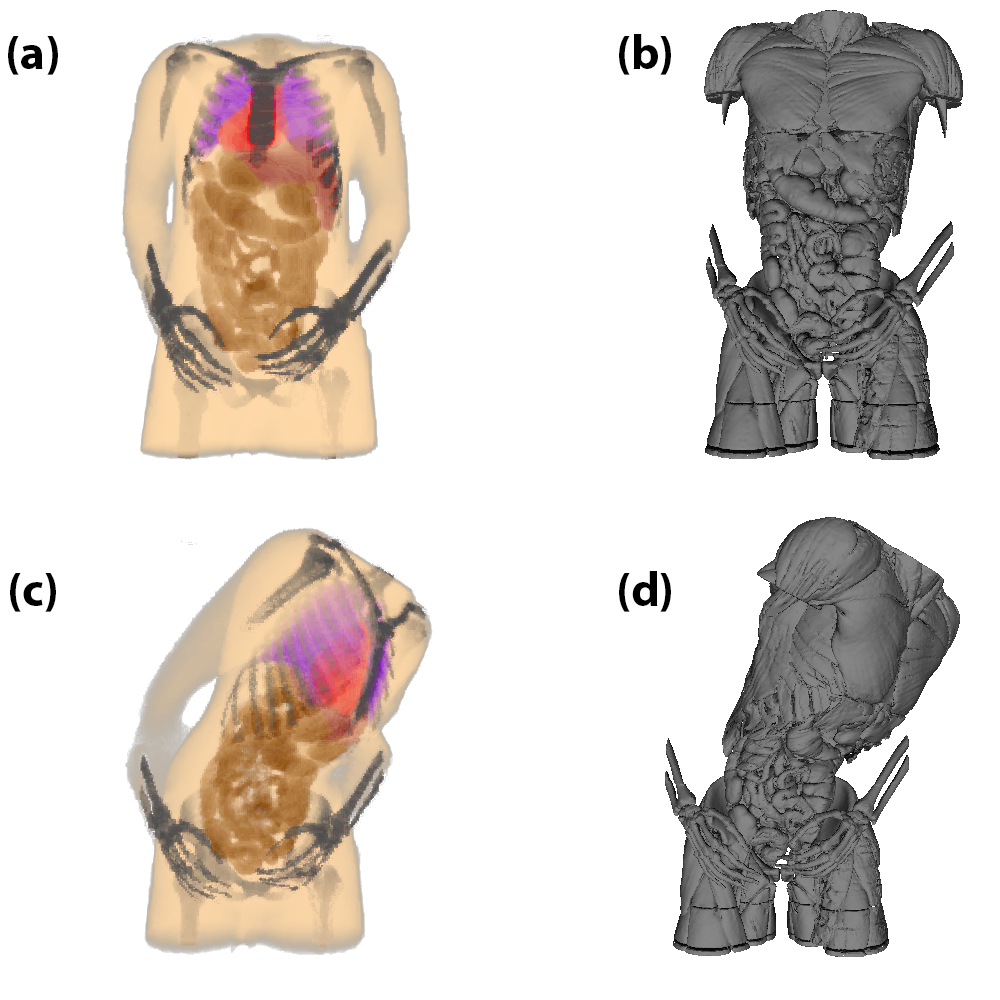
\includegraphics[width=0.4\textwidth]{IMG/HV}
    \caption{Algoritmo aplicado a diferentes representaciones: volumétrica (a) y (c), superficial (b) y (d). Imágenes (a) y (b) muestran el \emph{Segmented Inner Organs} en posición de reposo. Imágenes (c) y (d) muestran el resultado del modelo deformado.}
    \label{fig:humanvisible}
\end{figure}
Con la intención de seguir mostrando las capacidades del algoritmo propuesto, se presentan más ejemplos de deformaciones realizadas para esta tesis. En la figura \ref{fig:humanvisible} podemos observar tanto el modelo superficial como el volumétrico de los datos del proyecto \emph{Segmented Inner Organs}(\cite{VM2002},~\cite{VoxelMan}).



%%%%%%%%%%%%%%%%%%%%%%%%%%%%%%%%%%%%% 








%Due to their high content of water, organic tissues can be considered incompressible. For that reason, volume conservation is a desirable feature. In this vein, we have compared the behaviour of LBS, DQS, CoR and our Optimization step (FEM). To this end, we used the same MoCap walk cycle to animate the previously mentioned models. The results of this test are shown in Fig.  \ref{fig:volRatio}.
%\textcolor{red}{It can be observed how the optimization stage solve the volume problems of LBS and DQS. VER QUE PASA CON COR. }
%\begin{figure*}%[!ht]
%   \centering
%    \includegraphics[width=0.98\textwidth]%{img/graficas}
%    \caption{Volumen conservation rate of %the several \emph{skinning} techniques. }
%     \label{fig:volRatio}
%\end{figure*}

\section{Discusión}
\label{posing:discusion}
\todo{Hablar de la necesidad de validación}


\todo{La palabra realista me suena poco cientifica. Plausibles es un resultado que un usuario pueda interpretar como real.  }
\del{A la vista de los resultados, se puede afirmar que el algoritmo propuesto cumple con la función de generar resultados visualmente \del{realistas}\new{plausible} que en el contexto de entrenamiento puede ser utilizadas para que la transferencia de habilidades de los simuladores que la utilicen sea efectiva. } \todo{Como puedes afirmar que estos resultados son validos para el entrenamiento!!!!!!!! Has entrenado a médicos y después lo has evaluado!!!!! Aaron cuidado con lo que pones. La hipótesis es esa porque el objetivo era probar este sistema en herramientas reales. Hasta que no haya resultados en un simulador la hipótesis no queda probada!!!!!}

Esta técnica permite generar una cantidad infinita de variaciones anatómicas de un mismo modelo. En ese sentido, esta herramienta va a ser utilizada para crear una base de datos de modelos virtuales que posteriormente podrá ser utilizada tanto por el proyecto \ac{RASimAs}, como por aquellos simuladores que puedan beneficiarse del reposición de modelos anatómicos que permite el algoritmo propuesto. En el capítulo siguiente, se describirá como se ha incluido la solución presentada en el desarrollo de la herramienta \ac{TPTVPH}.

Por otra parte, la técnica presentada en esta tesis también puede cumplir con la funcionalidad de animar pacientes virtuales en herramientas interactivas. Este método se puede incorporar en cualquier simulador que requiera cambiar la pose a un determinado modelo anatómico con estructuras internas en tiempo real. Para demostrar esta funcionalidad, se presentará en los capítulos siguientes un simulador de radiología diagnóstica que utiliza las ventajas del modelo propuesto.

\new{El algoritmo propuesto se diseñó con el objetivo de ser lo más flexible posible, minimizando los requisitos de los datos de entrada. La clave de está flexibilidad radica en que se calcula un campo de deformaciones interno. Este campo de deformaciones permite adaptar cualquier tejido a la pose deseada, de forma independiente al resto de tejidos, pudiendo así trabajar con modelos incompletos. En este sentido, la única limitación es que tanto la piel como el tejido oseo del paciente virtual deben de estar segmentados. Esta restricción no supone un gran problema dado que estos tejidos son visibles en la mayor parte de las técnicas de imagen médica.}

\new{La flexibilidad que aporta el calculo del campo interno de deformaciones, aporta beneficios adicionales. Tal y como se muestra en la sección \ref{XXXXX}, este campo puede aplicarse a estructuras representadas tanto mediante B-reps \todo{mete acrónimo} como datos volumétricos. Extendiendo de esta manera el alcance de la técnica propuesta. }

\new{Evitar colisiones y autocolisiones en los tejido transformados es de vital importancia de cara a garantizar el buen funcionamiento del simulador físico y del simulador de \ac{US} de \ac{RASimAs}. Con el objetivo de garantizar este requisito, el algoritmo propuesto calcula un campo de deformaciones continuo. De esta forma, solo podrán aparecer colisiones y/o autocolisiones si: (i) se utilizan mallas para representar los tejidos con una resolución inadecuada o (ii) si existen colisiones y/o autocolisiones en el modelo virtual de partida. Debido a que la extracción de los tejidos desde imágenes médicas no es perfecta, pueden aparecer las auto colisiones y colisiones entre tejidos. La técnica propuesta no solventa estas colisiones, pero es robusta en su tratamiento. Aun así, las colisiones con el tejido oseo y muy especialmente con la piel, pueden provocar una importante perdida de realismo. Cabe destacar, que, a pesar de esta circunstancia, la técnica propuesta es mucho más robusta, en este escenario, que los métodos basados en simulación física. En la sección \ref{XX}, se proponen técnicas para mitigar estos problemas.}




